\documentclass{standalone}
\usepackage{tikz}
\usepackage{../mss}
\usepackage{sansmath}


\usetikzlibrary{shapes.geometric,positioning,calc,petri,graphs,fit,backgrounds}
\tikzset{
    node distance=1cm and 2.0cm,
    >=latex,
    font=\sf\bfseries\sansmath,
    ,
    textfeld/.style={align=center,minimum height=0.5cm,minimum width=1.5cm},
    pfeil/.style={->,line width=1.1pt},
    dot/.style={circle, fill, inner sep=0.2mm, outer sep=0.2mm},
    marking/.style={align=center,inner sep=1pt},
    box/.style={rectangle,draw,line width=1.1pt,minimum height=1.5cm,minimum width=2.8cm,align=center},
    place/.style={circle,line width=1.1pt,draw=black,minimum size=6mm},
    transition/.style={rectangle,line width=1.1pt,draw=black,minimum size=6mm},
    segment/.style={rectangle,draw,dashed,rounded corners=3mm,minimum height=1.5cm,minimum width=1.5cm},
    generator/.style={rectangle,draw,fill=gray!5,dashed,rounded corners=3mm,minimum height=1.5cm,minimum width=1cm},
    every edge/.append style={line width=1.1pt},
}
\tikzgraphsset{
    every graph/.style = {use existing nodes}
}

\begin{document}
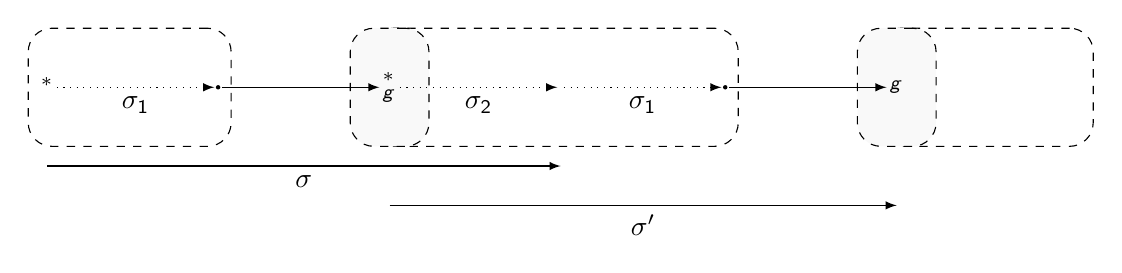
\begin{tikzpicture}
    \node[marking](m*)  {$ \marking^* $};
    \node[dot,right=of m*] (mas1){} ;

    \node[marking,right=of mas1](mg*)  {$ \marking_g^* $};
    \node[marking,right=of mg*](m)  {$ \marking $};
    \node[dot,right=of m] (mas2){} ;

    \node[marking,right=of mas2](mg)  {$ \marking_g $};

    \node[right=of mg](anonymous)  {};

    % sigma
    \draw[->,dotted] (m*) -- node[below] {$\sigma_1$} (mas1);
    \draw[->] (mas1) -- node[below] {$\synchronization$} (mg*);
    \draw[->,dotted] (mg*) -- node[below] {$\sigma_2$} (m);
    \draw[->] ($(m*)+(0,-1.0)$) -- node[below] {$\sigma$} ($(m)+(0,-1.0)$);

    % sigma prime
    \draw[->,dotted] (m) -- node[below] {$\sigma_1$} (mas2);
    \draw[->] (mas2) -- node[below] {$\synchronization$} (mg);
    \draw[->] ($(mg*)+(0,-1.5)$) -- node[below] {$\sigma^\prime$} ($(mg)+(0,-1.5)$);

    \begin{scope}[on background layer]
        \node[segment, fit=(m*)(mas1)] (o1) {};
        \node[segment, fit=(mg*)(m)(mas2)] (o2) {};
        \node[segment, fit=(mg)(anonymous)] (o3) {};
        \node[generator, fit=(mg*)] (g2) {};
        \node[generator, fit=(mg)] (g3) {};
    \end{scope}

\end{tikzpicture}
\end{document}
